\chapter{Conceptos básicos}

\label{BasicConcepts}

\section{Convoluciones}

Una imagen en el ámbito digital se entiende como una matriz de puntos.
Cada uno de estos puntos puede ser interpretado como un número, que representa la localización de este punto en la escala de grises. En este modelo cada elemento será un número entre 0 y 1, 0 representando el extremo oscuro de la escala y 1 el extremo claro.
Para imágenes en color, si se usa el modelo RGB (Red, Green, Blue), cada uno de estos puntos de la matriz es representado por tres números, correspondientes a la escala en cada uno de los colores primarios de RGB.

Por lo tanto, una imagen como la siguiente:
\begin{center}
  
\includegraphics{Seven_corner}
 % \makebox[\textwidth]{
\includegraphics[width=\linewidth]{Seven_corner}}
\end{center}

Sería representada por esta matriz.

\begin{center}
  \makebox[\textwidth]{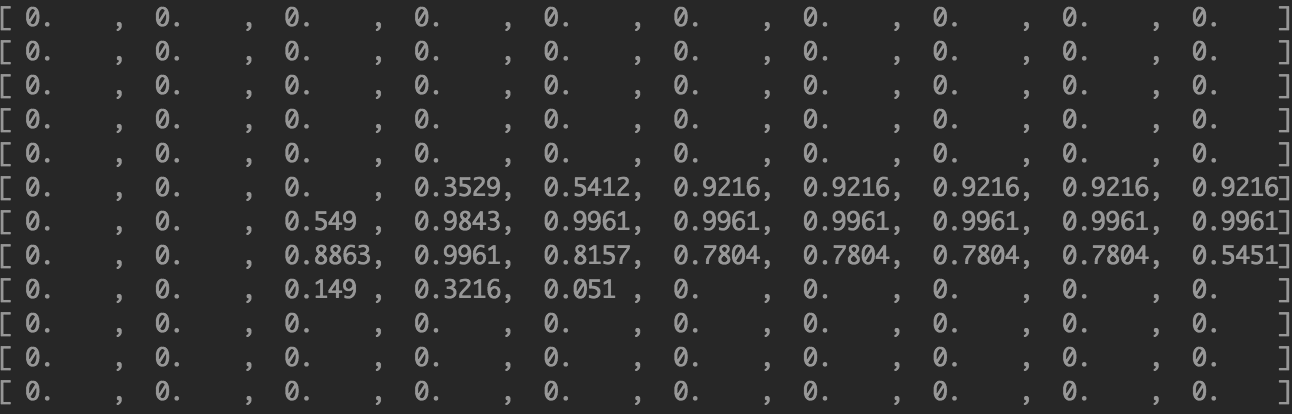
\includegraphics[width=\linewidth]{Seven_number}}
\end{center}

Para simplificar, la mayoría de los ejemplos van a usar una escala de grises, pero son aplicables a imágenes RGB aplicando las operaciones a las tres diferentes capas al mismo tiempo.

\subsection{Filtros}

Al trabajar con esta interpretación de lo que es una imagen, se pueden usar operaciones sobre la matriz de la imagen para transformarla de diferentes maneras.

Imaginemos una matriz de 3x3:

\[
  F=
  \left[ {\begin{array}{ccc}
   -1 & -1 & -1 \\
   1 & 1 & 1 \\
   0 & 0 & 0 \\
  \end{array} } \right]
\]

Se puede usar la matriz como un filtro para la imagen I de la siguiente manera: Primero, superponemos la matriz en algún punto de la imagen I. Esto modificará el pixel donde ha quedado colocado el valor central de la matriz F.  Multiplicamos cada uno de los valores superpuestos, sumamos los resultados y los sustituimos en el valor central. Si hacemos esto para cada píxel de la imagen original (superponer el filtro en ese píxel y sustituir el valor por la operación), la imagen cambiará.

En el caso de la matriz F, la fila superior son todos valores negativos, la intermedia son todos 1 y la inferior todos ceros. Si aplicamos la operación descrita con la matriz F sobre una imagen, los píxeles más brillantes (aquellos con mayor valor) serán los que su fila superior es cero, eliminando los valores negativos y la fila intermedia es 1. Esto ocurrirá con más frecuencia en los bordes superiores de objetos claros con fondo oscuro.

Para ver la utilidad vamos a verlo aplicado a la imagen de un dígito escrito a mano, sacado del dataset MNSIT (cita req).
\begin{center}
  
\includegraphics{seven}
\end{center}

Si aplicamos el filtro a la imagen podemos observar como resalta en blanco los bordes superiores y en negro los inferioes. Filtros similares, rotando los valores del filtro F, son capaces de resaltar bordes lateras u oblicuos.

\begin{center}
  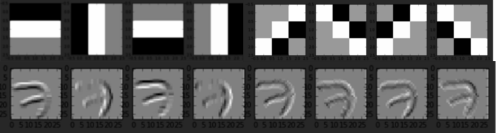
\includegraphics{filters}
\end{center}

Lo interesante de este método es que hemos conseguido resaltar características del objeto representado en la imagen solo multiplicando matrices.

Para ver como afectan diferentes filtros a una imagen, existe una página (http://setosa.io/ev/image-kernels/ mover a biblio) donde se pueden probar ejemplos con filtros personalizados, haciendo el concepto mucho más sencillo de comprender.


